%第3-1章
\section{感染症予防サポートシステムの概要}
本節では、はじめに感染症予防サポートシステムの開発の目的について説明した後、それを実現するための手段、開発を進める際の課題について述べ、実際に開発したシステムの概要について説明する。

まず私たちは、システムを開発するにあたって、本研究で開発するシステムの目的を定めるところから始めた。何よりもこのシステムで実現しなければならないことをメンバー同士で議論し合った結果、1章で述べたように、世界的な感染拡大が続く新型コロナウイルスへの感染予防対策の一環として取り組むべきとされている、3密の回避のサポートを第一の目的とした。具体的には、学校の教室などの、数人から数十人程度が利用するような部屋で稼働させることで、その部屋に入室可能な人数の目安を示し、部屋の警戒レベル・感染リスクを分析することで、密閉を防ぎつつ、状況に応じて部屋に滞在可能な人数を段階的に制限することによって、その部屋に滞在する人々を3 密の危険から守ることを想定し、システム開発を進めることとなった。続いて私たちは、この目的を実現するためにシステムが果たすべき役割として、以下の2つが挙げられると考えた。


\begin{itemize}
	\item 感染症予防対策のルールを守ってもらうよう働きかける役割
	\item 感染症予防対策の基準を定める役割
\end{itemize}

少なくともこれら2つの役割を満たして、はじめてこのシステムが利用者による3密回避のための行動をサポートできると考えた。3密の回避においては、「密閉」「密集」「密接」の3つの要素が関与することから考えても、上に示した2つの役割を果たすシステムの開発を行うには、その方法を十分に議論する必要があったが、実際の詳細な設計に関しては後で述べる。

続いて本研究で開発するシステムが、先ほど述べた2つの役割を果たすためには、どのような働きを持つべきかを議論した。

まず、利用者に感染症予防対策のルールを守ってもらう役割を果たすには、利用者の感染症予防対策への取り組みの状況を、利用者自身が把握できる必要があると考えた。つまり、リアルタイムで部屋の利用者の感染症予防対策の取り組みを監視し、現在の取り組みがルールに即したものであるかどうかの度合いを知らせ、ルールに反している場合には警告を出すなどし、利用者に感染症予防対策を促すような機能が求められると考えた。

また、感染症予防対策の基準を定める役割を果たすためには、リアルタイムな環境モニタリングによる、総合的な環境分析から得られる結果に基づいた基準を定める必要があると考えた。ここでは、環境の監視と分析の2つの機能が必要となり、環境の監視からどのような情報が得られ、その情報が分析の機能によって、どう意味付けされ、分析の結果得られる情報が感染症予防対策に、どう反映されるべきかを考える必
要がある。

このように、本研究で開発するシステムには、監視と分析という2つの機能が必要になる。これらの機能について、機能を実現する際の方針と課題について述べる。

\subsubsection*{監視の機能}

まず監視の機能については、どのような情報をどのようにして収集するかを考えた。まず3つの密のうち、「密閉」を避けるためには部屋の換気状況を監視する必要がある。こちらは、部屋に人が滞在している状況で、部屋の空気の入れ替えが十分に行われているかどうかを把握できれば良いため、室内の二酸化炭素濃度の高さを監視することによって、状態を把握できると考えた。

ここで考慮しなければならないのが、適切に部屋の換気状況を調べるためには、どのような場所に何台のセンサデバイスを設置すればよいかである。二酸化炭素は気体の一種であるため、部屋中に一様に広がっているわけではなく、同じ部屋の中でも場所によって、微妙に濃度が異なるはずである。したがって、部屋の中心に1台のセンサデバイスを設置しただけでは、室内の二酸化炭素濃度を適切に計測したことにはならないため、部屋の広さに応じてセンサデバイスを、複数台設置する必要があると考えた。ただし、ここで用いるセンサデバイスには、1章でも述べたように無線マイコンモジュールTWELITEを選定した。

「密集」「密接」を避けるためには、部屋に滞在する人の数を監視するだけでなく、部屋の広さに関する情報も必要となると考えた。また、ソーシャルディスタンスを保つために、何平方メートルに1人が滞在可能とするかといった、部屋の運用ルールも併せて考えることが、「密集」「密接」の回避のために扱う情報として適当であると考えられることから、部屋に関する情報も併せて分析の対象とすることとした。

部屋に滞在する人の数に関しては、室内にWebカメラを取り付けたマイコンを設置し、取得した室内画像に対し、物体検出の技術を用いることで、監視することが可能となる。ここで考慮すべき点は、Webカメラによって部屋全体の画像を取得するには、どのようにマイコンを設置しなければならないかという点と、画像識別のプログラム実行にかかる時間によって、監視のリアルタイム性が損なわれないかという点である。今回採用した物体検出の技術による人数推定の方法では、Webカメラによって取得する室内画像が室内全体を捉えていなくてはならない。本システムで想定している利用環境は、学校の教室などであるため、部屋の前方の壁に取り付けるのが、最も部屋全体を捉えるためには適している。反対に、部屋全体を捉えられるような場所にカメラを設置できない場合や、部屋が広すぎるために1台のカメラでは部屋全体を捉えられないという場合には、本システムの運用には適さないということになる。

なお、本システムにおける、物体検出技術による人物の検出機能には、検出精度のみならず、迅速に人物検出の結果を出力することが求められることから、GPUによる高速な処理を可能とする高価なマイコンが必要となる点や、複数箇所から撮影した複数枚の画像から、室内の人数を推定することの技術的な壁の高さから、Webカメラとマイコンの対を、1つの部屋に複数設置するということを本研究では行わない方向となっている。このような点から、本システムを運用する際に推奨される環境としては、数人から数十人程度で使われる、比較的小さな部屋で、なおかつ設置したカメラによって部屋全体を撮影できることが条件となる。ただし、ここで用いるマイコンには、1章でも述べたようにAIエッジ向けコンピュータとして知られるJetsonシリーズのJetson nanoを選定した。

\subsubsection*{分析の機能}

分析の機能に関しては、監視によって得られた情報から、より高い価値を持つ「感染予防対策に役立てられる情報」を導き出すための分析方法を議論した。

分析の機能でははじめに、二酸化炭素濃度の高さから、部屋の感染症に対する警戒レベルを導出する。二酸化炭素濃度が高くなるほど、部屋が密閉された状態になっていると考えられるため、部屋の警戒レベルは高く設定される。ここで考慮しなくてはならないのが、ある時間に取得した二酸化炭素濃度だけで部屋の換気状態を正しく分析できるかという点であり、データに多少のばらつきがみられる可能性から考えて、一定時間連続的に取った値をもとにして分析を行う必要があると考えた。

続いて、導出された警戒レベル毎に制限される、室内に滞在可能な人数と、実際に室内に滞在している人数とを比較し、感染リスクを導出する。警戒レベル毎の滞在可能人数には、上限と下限を設け、上限を超える場合には感染リスクが最高となり、下限から上限の範囲内であれば、室内の滞在人数を維持できるものとし、下限を下回る場合には、感染リスクを高めない範囲内で滞在人数を増やすことができる段階にあるものとして、3段階で感染リスクを評価する。ただし、警戒レベルの高さに関わらず、部屋の広さと部屋の運用ルールから求められる部屋の滞在可能規定人数を上回る場合には、感染リスクは最高となる。

このようにして、分析の機能では、室内環境の監視によって得られた情報をもとに、部屋の警戒レベルと感染リスクを評価する。

ここまで、本研究で開発するシステムの目的、機能を実現する際の方針と課題について述べてきた。ここからは、実際に開発したシステムの概要を説明する。

まず、本研究で開発するシステムを利用する際の簡単な流れを図\ref{systemflow}に示す。

\begin{figure}[H]
	\centering
	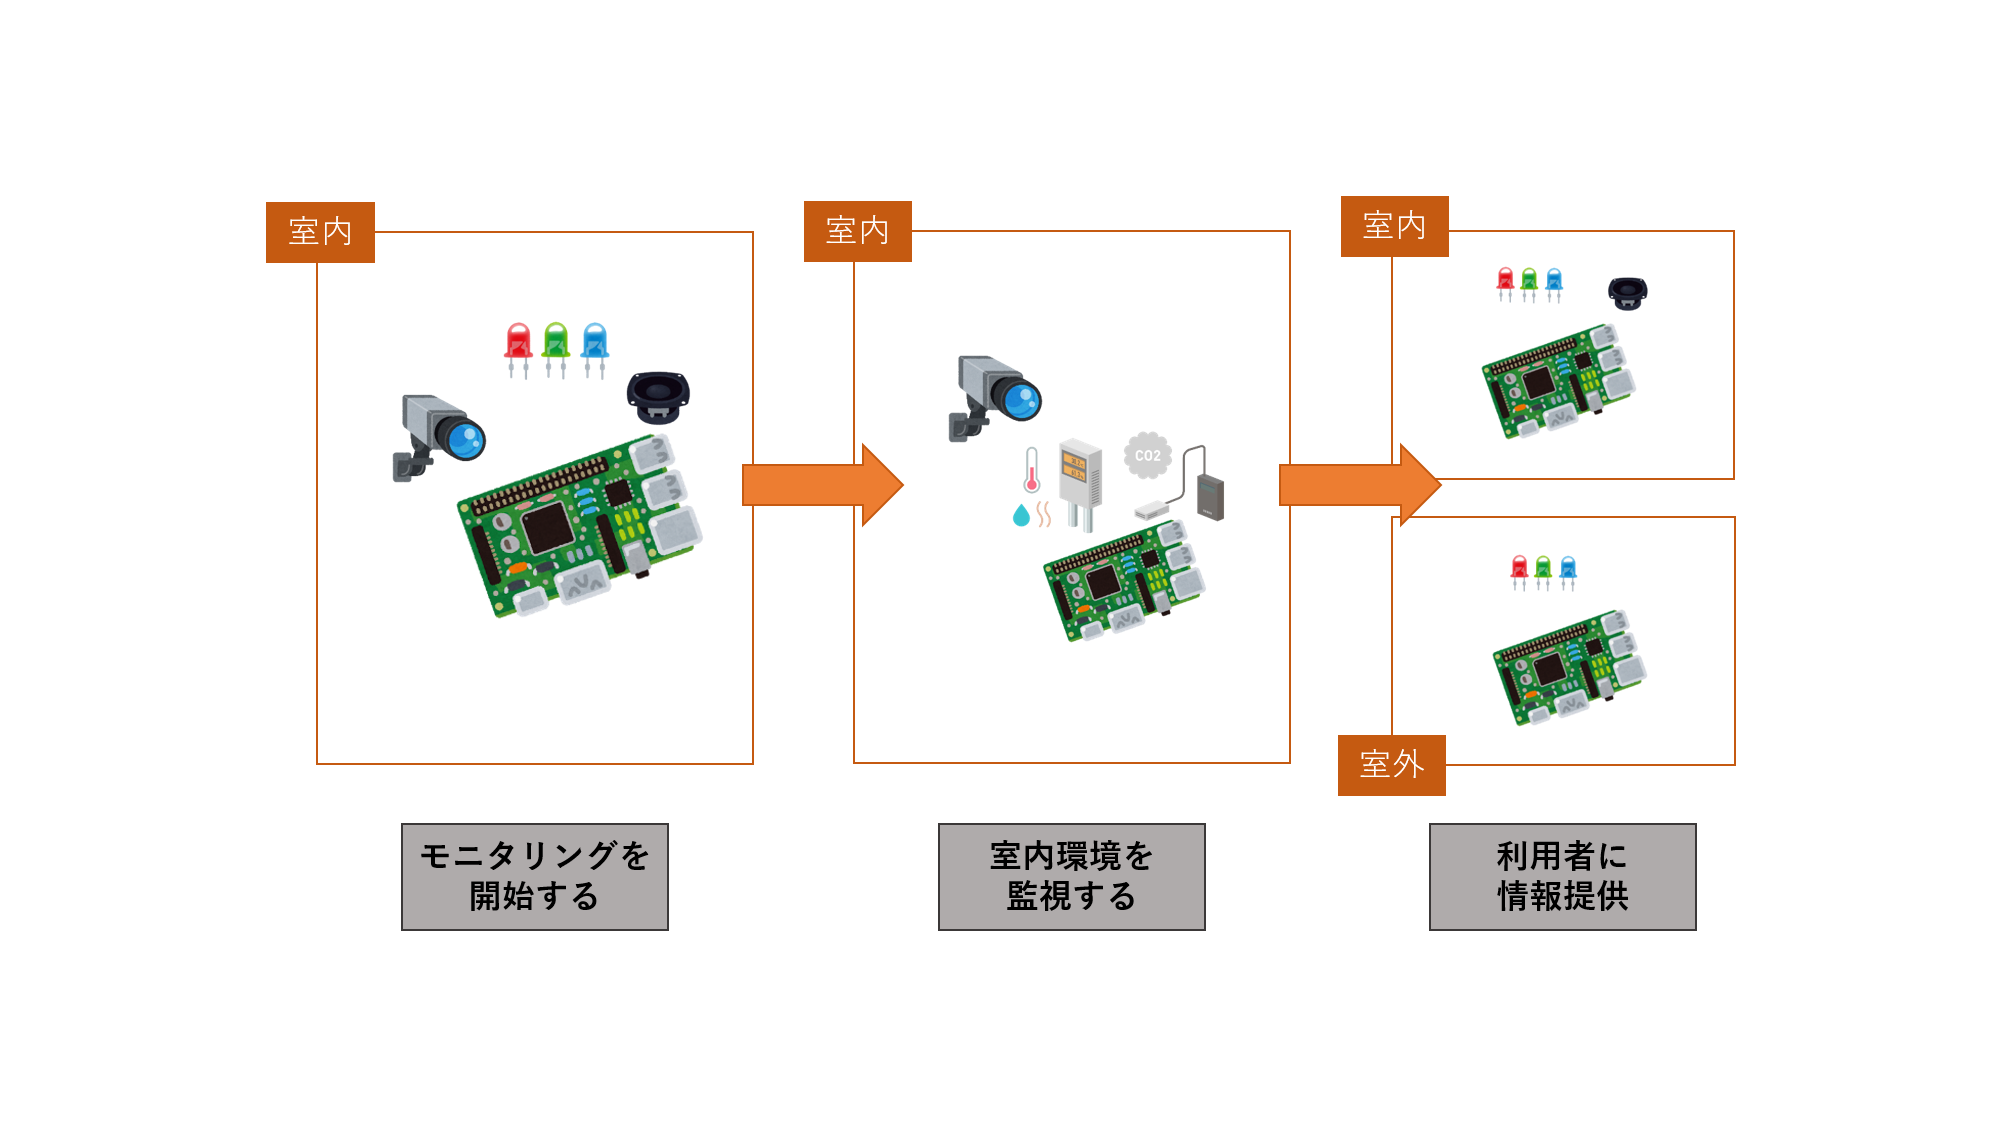
\includegraphics[width=15cm]{systemflow.eps}
	\caption{システム利用の流れ}
	\label{systemflow}
\end{figure}

まず、利用者はエッジサーバとしてシステム全体の中心となって稼働するJetson nanoに、部屋情報として、部屋の広さと何平方メートルに1人が滞在できるかという、部屋の運用ルールを登録する必要がある。感染予防サポートシステムを稼働させるには、このJetson nanoと、センサデバイスとして用いるTWE-LITEを室内に設置する。センサデバイスは部屋の広さなどに応じて、台数を増やすことが可能である。また室外には、部屋への入室の危険度を知らせるためのデバイスとして用いるTWE-LITEを設置する。あとは各デバイスの電源を入れ、エッジサーバであるJetson nanoによってモニタリングを開始するのみである。

デバイス類はシステム稼働後にそれぞれ接続され、基本的には3分おきに室内画像と、二酸化炭素濃度や温湿度といった環境値をそれぞれ、Jetson nanoに取り付けたWebカメラ、室内センサデバイスに取り付けたセンサ類によって取得し、それらのデータをJetson nanoで受け取った後、室内画像をもとにした人数推定と環境値をもとにした分析を行う。Jetson nanoでは、分析結果に基づき、換気要請や感染リスク状況をブザーとLEDを用いて、室内の利用者に通知する。また室外デバイスでは、Jetson nanoにより分析された部屋への入室危険度を受け取り、その都度リスクに応じたLEDを点灯する。これら一連の流れを8時から20時まで行い、夜間はスリープ状態に入るというのが、基本的なシステムの稼働の流れである。ここでシステム全体構造のイメージを図\ref{systemconst}に示す。

\begin{figure}[H]
	\centering
	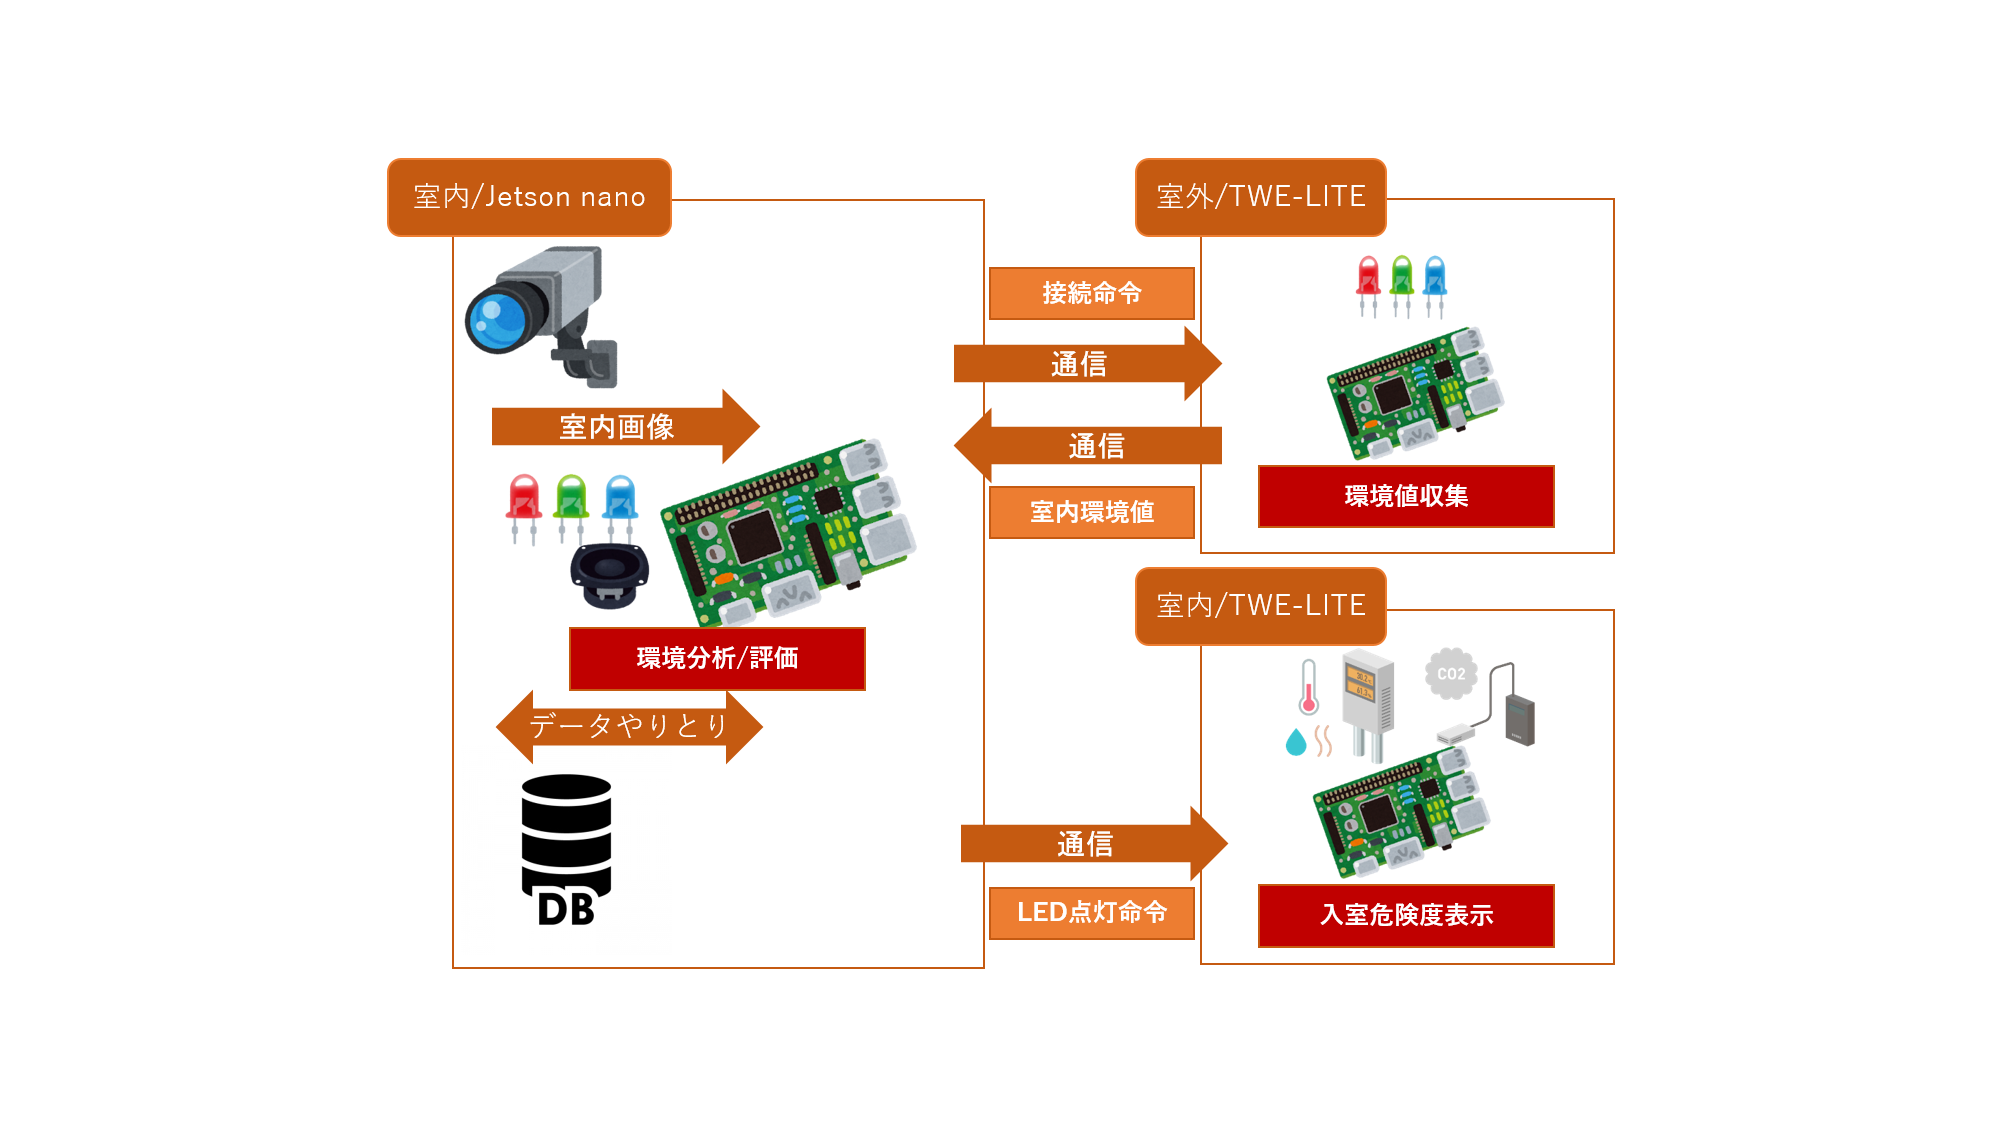
\includegraphics[width=15cm]{systemconst.eps}
	\caption{システム全体構造}
	\label{systemconst}
\end{figure}

なお本システムの開発は、エッジサーバ側を掛水誠矢が、センサデバイス側を稲田一輝が、室外デバイス側を小田恵吏奈が、人数推定機能を伊藤大輝が担当する。



